\chapter{Improving search efficiency}
\label{chap:approx}

We now turn our attention to the efficiency aspects of the neighborhood
similarity-search problem, \ie{}, the Problem~\ref{problem:neighborhood-search}
defined in \autoref{sub:neigh-problem}. The approach used to solve this problem so
far is an exhaustive search algorithm, as the one employed in the previous
chapter for the evaluation of neighborhood distance measures. Namely, given
neighborhood \region, consider all candidate neighborhoods $\region'$ of a
certain shape (circle, rectangle, or other) in the target city~$\city'$,
evaluate the distance $\mathrm{\emd}(\vfvs(\region),\vfvs(\region'))$, and
return the neighborhood that achieves the smallest distance. 

In this chapter, we present an alternative method to solve the same problem
(\autoref{sec:app-method}). Then we demonstrate experimentally that it
accelerates the search task significantly while incurring little loss in
accuracy over a wide range of parameters (\autoref{sec:app-result}).


\section{Method}
\label{sec:app-method}

Our solution relies on the following observation: the \emd\ between two sets
of feature vectors $\vfvs(\region)=\vfvs$ and $\vfvs(\region')=\vfvs'$ is zero,
if all feature vectors in \vfvs\ and $\vfvs'$ coincide. Relaxing this
condition, the \emd\ is small, if for many vectors in \vfvs\ there is some
\emph{near} vector in $\vfvs'$. Put differently, when one feature vector in \vfvs\
is \emph{far away} from all vectors in $\vfvs'$, it contributes a large cost to
\emd.

Therefore we can reduce the search space by preprocessing all venues in the
target city and keeping only those venues whose feature vectors are close to
feature vectors of venues in the query neighborhood. The venues kept in this
preprocessing step can be used as \emph{anchors}. We can then look for areas
in the target city that are dense in anchor venues, and group them in candidate
neighborhoods, for which we calculate the actual \emd{}.

\medskip

To see how this idea works, consider \autoref{fig:pigalle_barca}
\vpageref{fig:pigalle_barca}, 
where we search in Barcelona to find the neighborhood that is most
similar to Pigalle in Paris. 
Each row in the figure corresponds to one venue \venue\ in Pigalle, 
and contains the ranking of all venues in Barcelona sorted by distance to
\venue. 
There is a cross
\tikz{\draw (0,0) node[cross out, line width=0.4pt, draw=black,
		minimum size=2*(2.5pt-\pgflinewidth), inner sep=0pt,
outer sep=0pt] {};} in $i$\textsuperscript{th} position of the ranking if the
$i$\textsuperscript{th} ranked venue in Barcelona belongs to the ground truth
neighborhood.
We see that if we restrict ourselves to the 100 nearest neighbors of
each venue in the query neighborhood, 
we recover most of the venues in the ground-truth neighborhood.

\begin{figure}[b]
    \centering
    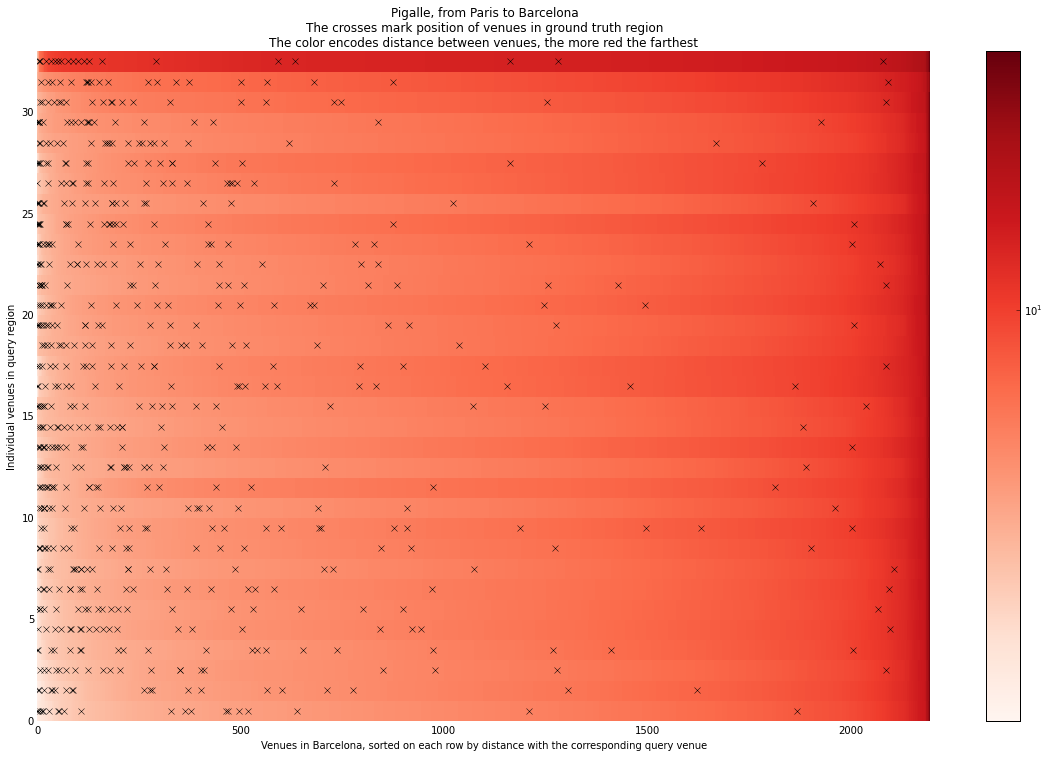
\includegraphics[width=1\linewidth]{pigalle_barca.pdf}
    \caption[Ranking of target city venues by distance to query
    venus.]{Intuition behind our pruning strategy: 
for two neighborhoods with small \emd, 
the venues of one neighborhood are in the $k$-NN set of the venues of
the other.  \label{fig:pigalle_barca}}
\end{figure}

We show the effect of varying $k$ in the experiments but first, we try to find
a good value a priori.  The larger $k$, the more venues we retrieve,
especially the more ground truth venues. But it also makes the search space larger,
because it covers a larger proportion of the city. This trade off is visualized
in \autoref{fig:coverage_recall} \vpageref{fig:coverage_recall}, where each point of each query is obtained
for a value of $k$ ranging from $1$ to $256$. We initially chose $k=50$
because in most cases, it returns 50\% of the ground truth venues while covering 33\%
of the city on average. These numbers hint that the precision is rather low and
we need another step to further reduce the search space.

\medskip

\begin{figure}[tb]
    \centering
    \includegraphics[width=1\linewidth]{coverage}
    \caption[Recall vs coverage of $k$ nearest neighbors]{Recall of the $k$
	    nearest neighbors as a function of the fraction of the total
	    venues in the target city, for $k$ varying between $1$ and $256$.
	    Each line is query from Paris to another city, indicated by its
	    color.\label{fig:coverage_recall}}
\end{figure}


In short, our algorithm works as follows. 
Starting from the query neighborhood \region\ and target city $\city'$
(or cities), 
we obtain the set of $k$-nearest neighbors
$\neighbors_k(\venue)\subseteq\venues(\city')$
for each venue $\venue\in\venues(\region)$.
All venues found in at least one $k$-NN set form the set of anchor
venues 
$\venues_A=\bigcup_{\venue\in\venues(\region)}\neighbors_k(\venue)$.
The set of anchor venues $\venues_A$ is then treated with respect to its
geographic coordinates: the \textsc{dbscan} algorithm is applied with initial
parameters of $\epsilon=210$ and $\mathrm{minPts}=18$.
Depending of the results, we recurse over large clusters with
stricter parameters or over the whole city with more flexible ones until enough
cluster candidates of sensible size are found.
Finally, to account for misses that may happen during the pruning phase, each
area considered is extended by adding to its boundaries a distance of $j\times
\frac{\hat{s}}{\ell}$ meters, where $j=0,\ldots,\ell$ and $\hat{s}$ is the
overall size the area. These extended areas are then treated as candidate
neighborhoods. At the end of the process, the algorithm returns the
neighborhood with the smallest distance (or top-$m$ smallest distances).

Note that although we focus on \emd{}---because we determine it is the most
suited metric to match human judgment---our method is independent of the
underlying metric as it plays a role only at the very end of the algorithm.
\clearpage

\section{Results}
\label{sec:app-result}
\subsection{How well it approximates exhaustive \emd{}}


Here, we quantify how well our proposed method
approximates a brute-force \emd\ search. 
We conduct our performance evaluation on the $248$ query
triplets $(\city, \region, \city')$ that were used in the analysis
shown in \autoref{tab:distance-comparisons}.

For each of these queries, we execute the brute-force search, as
described in \autoref{sub:region-evaluation}; namely, 
we compute the \emd\ for all circles $(\venue',\radius)$ centered at
regularly spaced venues $\venue'$ of $\city'$ and with radius $\radius\in\{200,
\allowbreak 275, \allowbreak 350, \allowbreak 425, \allowbreak 500\}$ meters.
We also execute the neighborhood similarity-search algorithm,
described above. 
We compare these two methods in terms of \emph{execution time} and
\emph{quality} of solution found. 
In particular, given a query  triple $(\city, \region, \city')$
let $\region_{{BF}}$ be the most similar neighborhood found by
the brute force and 
let $\region_{{A}}$ be the most similar neighborhood found by
the approximation method. 
Let the corresponding closest distances be
$D_{{BF}} = \mathrm{\emd}(\vfvs(\region),\vfvs(\region_{{BF}}))$
and 
$D_{{A}} = \mathrm{\emd}(\vfvs(\region),\vfvs(\region_{{A}}))$, 
respectively.
We  define the \emph{\Dratio{}} $\rho$ for that query
as  
\begin{equation*}
\rho = \frac{D_{{A}}}{ D_{{BF}} }
\end{equation*}
The smaller is $\rho$, the better the approximation.
We would in fact expect $\rho$ to be greater than $1$, as values less
than $1$ indicate that the approximation method is better than the brute
force.
However, as the brute force is constrained to circular neighborhoods,
it is possible that the approximation method finds better solutions.
Removing this constraint from the brute force implies searching
over other shape families (rectangles, diamonds, etc.), which will
increase its running time even more.

\medskip

Overall, our results show that for the range of parameters we
experiment with, the approximation method is much faster than the brute
force---in most cases by at least one order of magnitude, while
often by two or even three.
At the same time the \Dratio{} is very close to $1$, often below $1$,
and rarely above $1.5$.

The two parameters of the algorithm, $k$ and $\ell$, offer an accuracy vs.\
efficiency trade-off, that we illustrate empirically.
In more detail, we first analyze the effect of $\ell$, the number of times we
extend the initial regions found after clustering, while using our initial
estimate $k=50$. 
Intuitively, as $\ell$ increases, more \emd\ computations are required, but the
chances to find a more similar region increase. Indeed, as we see in
\autoref{fig:distance_ratio_size} \vpageref{fig:distance_ratio_size}, 
the relative distance decreases as $\ell$ increases while the
computation becomes more expensive (\autoref{fig:time_ratio_size}). 
We also note that after $\ell=1$, the gain is small, suggesting that
the initial regions are already relevant enough.

\begin{figure}[t]
    \begin{subfigure}[b]{\linewidth}
        \centering
        \includegraphics[width=\linewidth]{ratio_size}
		\caption[\Dratio{} as $\ell$ increases]{Box plot of the \Dratio{} between
          nearest neighbor \emd\ computed by the approximation
          method and brute-force, as $\ell$ varies.
          Values smaller than 1 indicate that the approximation method
          finds a neighborhood with smaller distance than the brute force. 
	\label{fig:distance_ratio_size}}
    \end{subfigure}

    \begin{subfigure}[b]{\linewidth}
        \centering
        \includegraphics[width=\linewidth]{speedup_size}
	\caption[Time speed-up as $\ell$ increases]{Time speed-up for each query, in
          descending order. Note the logarithmic scale.\label{fig:time_ratio_size}}
    \end{subfigure}
    \caption[Approximation trade off with respect to $\ell$]{Approximation
    trade off while expanding the size of the regions
    considered.\label{fig:approx_by_size}}
\end{figure}

We perform the same experiment for $k \in \{8, 25, 50, 80, 160\}$ with
$\ell=1$.  As shown in \autoref{fig:distance_ratio_knn}
\vpageref{fig:distance_ratio_knn}, the \Dratio{} is very
small for all values of $k$, showing the robustness of the method.  At the same
time, the running time increases somewhat (\autoref{fig:time_ratio_knn}), but
this is due to regions being denser and thus \emd{} taking more time to reach a
solution of the optimization problem.

\begin{figure}[t]
        \centering
    \begin{subfigure}[b]{\linewidth}
        \includegraphics[width=\linewidth]{ratio_knn}
		\caption[\Dratio{} as $k$ increases]{Same as
			\autoref{fig:distance_ratio_size} but showing the effect of varying
			$k$.  \label{fig:distance_ratio_knn}}
    \end{subfigure}

    \begin{subfigure}[b]{\linewidth}
        \centering
        \includegraphics[width=\linewidth]{speedup_knn}
	\caption[Time speed-up as $k$ increases]{Same as
			\autoref{fig:time_ratio_size} but showing the effect of varying
			$k$.\label{fig:time_ratio_knn}}
    \end{subfigure}
    \caption[Approximation trade off with respect to $k$]{Approximation trade
	    off while expanding $k$, the number of nearest neighbors of each
    query venues.\label{fig:approx_by_knn}}
\end{figure}

\subsection{How well it matches ground truth}

The method we devise finds neighborhoods that generally have comparable
distance to the query as those found by exhaustive search, but are obtained
much faster.
Yet we also want to see if these new neighborhoods retain another
characteristics of the exhaustive search: to be close to human ground
truth. To answer that, we can perform the same evaluation as in
\autoref{sub:region-evaluation}. Results showed in \autoref{tab:approx-adcg}
\vpageref{tab:approx-adcg}
indicates that if we sort obtained neighborhood by \emd{} distance, they
perform worse than exhaustive search. Yet the last column shows that among
the remaining neighborhoods, some are indeed overlapping with the ground truth.
These mixed results can be explained by two problems:
\begin{itemize}
	\item Sometime, there are too few close neighbors in the ground truth
		region to form a cluster. Since it was our main assumption, we cannot
		expect our approximation to return these regions.
	\item Alternatively, there is a cluster in the ground region but some
		clusters elsewhere have smaller \emd{} distance. But this case
		represents more a failure of \emd{} to recognize ground truth region and simply
		indicates that our approximation method cannot alleviate this
		shortcoming.
\end{itemize}

\begin{table}[t]
	% \small
	% \setlength{\tabcolsep}{4pt}
	\centering
	\begin{tabular}{lccc}
		\toprule
		              & Approximation & Exhaustive & Biased Approximation \\
		\midrule
		Barcelona     & $0.066$       & $0.075$       & $0.170$ \\
		New York      & $0.029$       & $0.057$       & $0.132$ \\
		Paris         & $0.067$       & $0.091$       & $0.191$ \\
		Rome          & $0.023$       & $0.038$       & $0.070$ \\
		San Francisco & $0.044$       & $0.045$       & $0.082$ \\
		Washington    & $0.071$       & $0.035$       & $0.161$ \\
		\midrule
		Average       & $0.050$       & $0.057$       & $0.134$ \\
		\bottomrule
	\end{tabular}
	\caption[Approximation ability to recover ground truth]{Average score when
		query are issued from the city on the left. The last row is the average
		score over all cities. The first column is the score obtained when
		taking the $5$ neighborhood with the smallest distance as returned by
		the approximation method. The second is the result of exhaustive
		search.  In the last one, neighborhoods are ordered to maximize the
		score. \label{tab:approx-adcg}}
\end{table}
